\documentclass[12pt]{article}
\usepackage[margin=2.5cm]{geometry}
\usepackage{enumerate}
\usepackage{amsfonts}
\usepackage{amsmath}
\usepackage{fancyhdr}
\usepackage{amsmath}
\usepackage{amssymb}
\usepackage{amsthm}
\usepackage{mdframed}
\usepackage{graphicx}
\usepackage{subcaption}
\usepackage{adjustbox}
\usepackage{listings}
\usepackage{xcolor}
\usepackage{booktabs}
\usepackage[utf]{kotex}
\usepackage{soul}
\usepackage{hyperref}

\definecolor{codegreen}{rgb}{0,0.6,0}
\definecolor{codegray}{rgb}{0.5,0.5,0.5}
\definecolor{codepurple}{rgb}{0.58,0,0.82}
\definecolor{backcolour}{rgb}{0.95,0.95,0.92}

\lstdefinestyle{mystyle}{
    backgroundcolor=\color{backcolour},
    commentstyle=\color{codegreen},
    keywordstyle=\color{magenta},
    numberstyle=\tiny\color{codegray},
    stringstyle=\color{codepurple},
    basicstyle=\ttfamily\footnotesize,
    breakatwhitespace=false,
    breaklines=true,
    captionpos=b,
    keepspaces=true,
    numbers=left,
    numbersep=5pt,
    showspaces=false,
    showstringspaces=false,
    showtabs=false,
    tabsize=1
}

\lstset{style=mystyle}

\pagestyle{fancy}
\renewcommand{\headrulewidth}{0.4pt}
\rhead{CSC369 Assignment 2}

\begin{document}
\title{CSC369 Assignment 2 - Page Tables and Replacement Algorithms}
\maketitle

\bigskip

\section{Introduction}

\bigskip

For this assignment, we're going back to the realm of user mode programming.
Specifically, you will have to simulate the operation of page tables and page
replacement. As I keep saying: the way to gain a solid understanding of the theory
is by applying it in practice.

\bigskip

\noindent You have two tasks in this assignment, which will be based on a \hl{virtual memory}
simulator. The first task is to implement \hl{virtual-to-physical address translation}
and hl{demand paging} using a \hl{two-level page table}. The second task is to implement
four different page replacement algorithms: \hl{FIFO}, \hl{Clock}, \hl{exact LRU}, and \hl{OPT}.

\bigskip

\noindent Before you start work, you should complete the set of readings about memory, if
you haven't done so already: \href{http://pages.cs.wisc.edu/~remzi/OSTEP/vm-paging.pdf}{link}

\bigskip

\section{Requirements}

\bigskip

\subsection{Setup}

\bigskip

\noindent You will find the starter code \href{https://www.teach.cs.toronto.edu//~csc369h/summer/assignments/new-a2/starter.zip}{HERE}.
It is your responsibility this time to add the code in your repository and make
sure that you submit all the necessary files!

\bigskip

\noindent Note that you may be generating some large trace files and must NOT commit any of
the trace files that you generate to your repository or you will run into serious
problems with disk quota. Most of the trace programs should be familiar to you from
the exercise in week 6. We have added a blocked version of matrix multiply, \textit{blocked.c}
which should exhibit fewer page faults under at least some of the page replacement
algorithms. The Makefile shows you exactly how to compile and run the traces. Note
that it takes quite a while to run the trace collection.

\bigskip

\noindent \textit{Compile the trace programs and generate the traces.}

\bigskip

\noindent You may have noticed while doing the Exercise that the traces generated
by Valgrind are enormous since they contain every memory reference from the entire
execution. We have provided a program, \textit{fastslim.py} to reduce the traces by removing
repeated references to the same page that occur within a small window of each other
while preserving the important characteristics for \hl{virtual memory} simulation.
(For example, a sequence of references to pages A and B such as "ABABABABAB...AB"
are reduced to just "AB".) The runit script pipes the output of valgrind through
this program to create the reduced trace. If you wish, you can experiment with
fastslim.py to try omitting the instruction references from the trace or using a
smaller or larger window (\textit{fastslim.py --help}). You may also want to create traces
from other programs, and you will definitely want to create small manual traces
for testing.

\subsection{Task 1 - Address Translation and Paging}

\bigskip

\textit{Implement \hl{virtual-to-physical} address translation and demand paging using a
two-level pagetable.}

\bigskip

\noindent The main driver for the memory simulator, \textit{sim.c}, reads memory reference traces in
the format produced by the fastslim.py tool from valgrind memory traces. For each
line in the trace, the program asks for the simulated physical address that
corresponds to the given virtual address by calling find\_physpage, and then reads
from that location. If the access type is a write ("M" for modify or "S" for store),
it will also write to the location. You should read sim.c so that you understand how
it works but you should not have to modify it..

\bigskip

\noindent The simulator is executed as \textit{./sim -f \textless tracefile\textgreater  -m \textless memory size\textgreater  -s \textless swapfile size\textgreater
-a \textless replacement algorithm\textgreater}  where memory size and swapfile size are the number of
frames of simulated physical memory and the number of pages that can be stored in
the swapfile, respectively. The swapfile size should be as large as the number of
unique virtual pages in the trace, which you should be able to determine easily.

\bigskip

There are four main data structures that are used:

\bigskip

\begin{enumerate}[1.]
    \item \textit{char *physmem}: This is the space for our simulated \hl{physical memory}.
    We define a simulated page size (and hence frame size) of \textit{SIMPAGESIZE} and
    allocate \textit{SIMPAGESIZE * "memory size}" bytes for \textit{physmem}.
    \item \textit{struct frame *coremap}: The coremap array represents the state
    of (simulated) physical memory. Each element of the array represents a physical
    page frame. It records if the physical frame is in use and, if so, a pointer
    to the page table entry for the virtual page that is using it.
    \item \textit{pgdir\_entry\_t pgdir[PTRS\_PER\_PGDIR]}: We are using a two-level page table design; the top-level is referred to as the page directory, which is represented by this array. Each page directory entry (pde\_t) holds a pointer to a second-level page table (which we refer to simply as page tables, for short). We use the low-order bit in this pointer to record whether the entry is valid or not. The page tables are arrays of page table entries (pte\_t), which consist of a frame number if the page is in (simulated) physical memory and an offset into the swap file if the page has been written out to swap. The format of a page table entry is shown here: image of pte format

    \bigskip

    Note that the frame number and status bits share a word, with the low-order
    \textit{PAGE\_SHIFT} bits (12 in our implementation) used for status (we only
    have 4 status bits, but you can add more if you find it useful). Thus, for a
    given physical frame number (e.g. 7), remember to shift it over to leave room
    for the \hl{status bits} (e.g., 7 \textless \textless \textit{PAGE\_SHIFT}) when storing into
    the pte and to shift it back when retrieving a frame number from a \hl{pte}
    (e.g., \textit{p-\textgreater frame \textgreater \textgreater PAGE\_SHIFT}).

    \begin{center}
    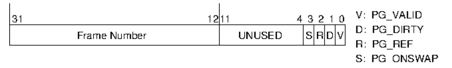
\includegraphics[width=0.8\linewidth]{../images/assignment_2_1.png}
    \end{center}


    \item \textit{swap.c}: The swapfile functions are all implemented in this
    file, along with \hl{bitmap} functions to track free and used space in the swap
    file, and to move virtual pages between the swapfile and (simulated)
    \hl{physical memory}. The \textit{swap\_pagein} and \textit{swap\_pageout}
    functions take a frame number and a swap offset as arguments. Be careful not
    to pass the frame field from a \hl{page table} entry (\hl{pte\_t}) directly, since that
    would include the extra status bits. The simulator code creates a temporary
    file in the current directory where it is executed to use as the swapfile,
    and removes this file as part of the cleanup when it completes. It does not,
    however, remove the temporary file if the simulator crashes or exits early
    due to a detected error. You must manually remove the swapfile.XXXXXX files
    in this case.
\end{enumerate}

\bigskip

\noindent To complete this task, you will have to write code in \textit{pagetable.c}. Read the code
and comments in this file -- it should be clear where implementation work is
needed and what it needs to do. The rand replacement algorithm is already implemented
for you, so you can test your translation and paging functionality independently
of implementing the \hl{replacement algorithms}.

\subsection{Task 2}

\bigskip

\noindent Using the starter code, implement each of the four different page replacement
algorithms: \hl{FIFO}, exact \hl{LRU}, \hl{CLOCK} (with one ref-bit), \hl{OPT}.

\bigskip

\noindent You will find that you want to add fields to the struct frame for the different
page replacement algorithms. You can add them in \textit{pagetable.h}, but please label
them clearly.

\bigskip

\noindent Once you're done implementing the algorithms, run all three programs from the
provided traceprogs, plus a fourth program of your choosing with interesting memory
reference behaviour, using each of your algorithms (include rand as well). For each
algorithm, run the programs on memory sizes 50, 100, 150, and 200. Use the data
from these runs to create a set of tables that include the following columns.
 (Please label your columns in the following order,)

\bigskip

\begin{itemize}
    \item Hit rate
    \item Hit count
    \item Miss count
    \item Overall eviction count
    \item Clean eviction count
    \item Dirty eviction count
\end{itemize}


\subsection{Write up}

\noindent Include a file called README.pdf that includes the following information.

\begin{itemize}
    \item The tables prepared in Task 2
    \item One paragraph comparing the various algorithms in terms of the results
    you see in the tables.
    \item A second paragraph explaining the data you obtained for \hl{LRU} as the size
    of memory increases.
\end{itemize}

\bigskip

\underline{\textbf{Notes:}}

\bigskip

\begin{itemize}
    \item First-In First-Out (FIFO)
    \begin{itemize}
        \item Is the simplest page replacement algorithm $^{[1]}$
        \item FIFO suffers from \textbf{Belady's Anomaly}
    \end{itemize}
\end{itemize}

\bigskip

\underline{\textbf{Refernces:}}

\bigskip

\begin{enumerate}[1)]
    \item Geeks for Geeks: Page Replacement Algorithm in Operating Systems, \href{https://www.geeksforgeeks.org/page-replacement-algorithms-in-operating-systems/#:~:text=First%20In%20First%20Out%20(FIFO,queue%20is%20selected%20for%20removal.}{link}
\end{enumerate}

\end{document}